\section{Environment}

The task environment is a virtual graphical computer program for building virtual block structures using either a LEAP Motion or keyboard and mouse. The environment was developed with the use of jMonkeyEngine~\cite{Irene:2012}, an open source 3D game engine written in Java. The Software Development Kit that comes with the engine provides a high level interface for numerous 3D functions and data-structures (e.g. spatial manipulation, quaternions and 3D meshes) and also provides a high degree of control for developers by being completely compatible with the Java programming language. The environment has been developed for being a general interface were the components could be controlled either through the LEAP Motion or with the keyboard and mouse depending on a simple setting in a configuration file. Therefore most of the components of the environment are utilized by both control strategies. To manipulate the environment with the LEAP Motion device controllers have been developed that employ the LEAP Motion SDK.

\subsubsection{Environment}

The task environment is a virtual graphical computer program for building virtual block structures using either a Leap Motion or keyboard and mouse. 

\begin{figure}[H]
\centering
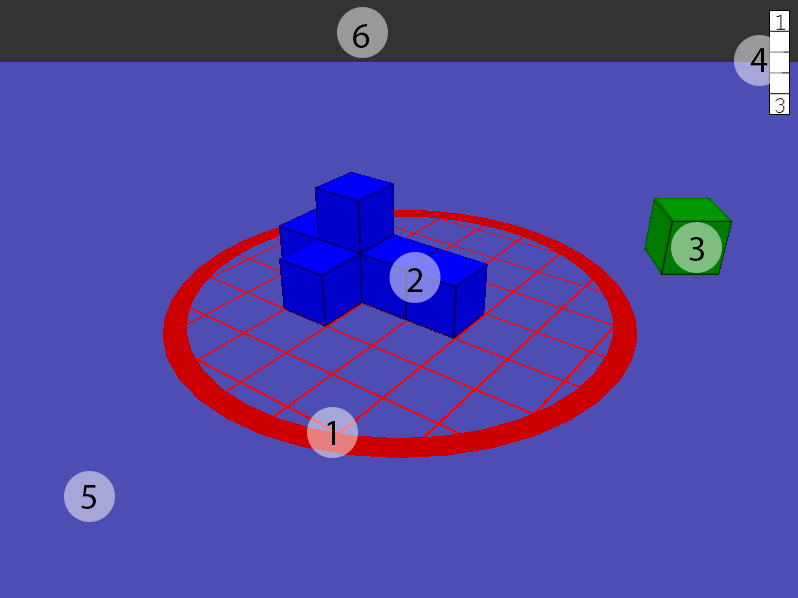
\includegraphics[width=\textwidth]{env_comps}
\caption{\label{fig:environmentcomps} Common rendering of the task environment. Visual elements: 1) Circular grid 2) Building blocks 3) Creation block 4) Target indicator 5) Floor 6) Horizon}
\end{figure}

\noindent Figure~\ref{fig:environmentcomps} shows a common rendering from the task environment where all groups of visual elements have been labeled. In the center of the screen users are presented with a circular grid that is segmented into several squares, effectively representing a grid with an circular border. On this grid building blocks can be positioned, either directly on the grid or stacked on top of other building blocks. New building blocks can be obtained by interacting (clicking with the mouse or grabbing with the Leap Motion) with the creation block outside the circular grid. The target indicator on the top right corner gives the user a representation of the block structure that should be created on the grid before the user can move further.

% Circular grid
% Creation block
% Building blocks
% Floor
% Horizon
% Target indication

\textbf{Design rationale}
The program was developed with the use of jMonkeyEngine, an open source 3D game engine written in Java. For development we used the Software Development Kit that comes with the engine, which provides a high level interface for numerous 3D functions and data-structures (e.g. spatial manipulation, quaternions and 3D meshes) and also provides a high degree of control for developers by being completely compatible with the Java programming language. 

Both the User Interface (UI) and the user interactions were designed to be minimalistic, simple and intuitive in order to prevent users having to learn a lot before they could use the system. 


\textbf{Does it work?}
\subsection{Control interfaces}\label{sec:interface}

The control interfaces define the actual control strategy, i.e. they describe the mapping from the input of a peripheral device towards the actual manipulations within the task environment. This section starts with a brief explanation of the two major sets of manipulations with the task environment and then discusses how these were implemented through control interfaces for the LEAP Motion and the mouse and keyboard. 

The major two sets of manipulations with the environment were:
\begin{enumerate}
	\item{\textbf{Building block manipulations:}} creating new blocks, dragging blocks, picking up blocks, dropping blocks and removing blocks.
	\item{\textbf{View manipulations:}} rotating the circular grid, lowering and raising the camera.
\end{enumerate}

\subsubsection{Keyboard and Mouse}

\paragraph{Building block manipulations}
In the keyboard and mouse interface, moving the block was solitary done with the mouse. To pick up a block the mouse button had to be clicked and held. As soon as the 
button was released, the block was also released. To move the block the mouse could be moved. However, to avoid flattening the environment to a 2D environment the movement 
of the mouse only determines the position in the 2D grid shown. To get the block higher, the scroll wheel of the mouse was used. The reason for doing this, is to make the 
comparison with the Leap Motion interface more fair. Because in the Leap Motion interface, there are also three dimensions in which the hand has to move.


\paragraph{View manipulations}
The view manipulations on the other hand were solitary done with the keyboard. In order to rotate the grid the left and right keys could be pressed respectively rotating the
 grid to the left or to the right at a constant pace. The up and down keys needed to be pressed in order to lift the camera up and down with a constant speed respectively.  
\subsubsection{Leap Motion}

\paragraph{Building block manipulation}
It was tried to keep the Leap M gesture as close to real life movements as possible. Therefore, the grabbing gesture had to be performed by closing a hand when it was 
shown above a block. The block was then shown inside the hand. While the hand remained closed the block would stay in the hand and move along with it. When the hand was opened 
the block would fall down at the position the hand was at that moment.

To indicate a grabbing gesture the function \texttt{Hand.scaleFactor(Frame sinceFrame)} from the Leap Motion SDK is used. This function looks at the scaling of the hand with 
all the fingers. When clenching the fist, the fingers get closer to the hand and therefore the scaling gets smaller, indicated by values $<1.0$. So for every frame, the program 
looks at the previous frame and finds a value of the scaling. When this value is lower than a certain threshold (in our case $<0.978$) it is saved. When the scaling gets lower 
for at least four frames, the system recognizes a grabbing gesture. When there are there are three or more frames in a row where the scaling is the same or bigger. The memory
 gets reset and the grabbing has to start over again.

After picking up it was easy to move the block, because the block would just follow the hand with which it was picked-up. Releasing was done in a similar manner as grabbing. 
When the scaling factor between the hand and the same hand in the previous frame was $>1.01$ for at least two frames the block got released. All thresholds were found with
 empirically.

An added feature to the Leap Motion interface was the fact that the hand should be near the block but not necessarily  on it to pick up the block. When detecting a grab gesture, 
the system would try to find a block within a certain parameter.

\paragraph{View manipulations}
The control of the circular grid through the Leap Motion is done by
swipe gestures. This choice was inspired by the numerous available
interaction patterns where swipe gestures are used to navigate through
some kind of interface. Also, a full hand swipe in a horizontal orientated
direction is similar to the movement one makes when spinning a plate
such as the circular grid. 

For these reasons a set of swipe gestures were implemented to rotate
the circular grid in both a horizontal and vertical direction (adjust
the angle at which the interface shows the grid). These gestures are
called the rotate gestures and are divided into two groups; swipe
gestures that move in a horizontal direction and those that move in
a vertical direction. The decision boundary lies at a $45$ degree
angle from the horizontal axis, any gestures beyond that angle are
classified as a vertical rotate gesture.

The straightforward implementation of these gestures based on the
swipe data presented by the Leap Motion and the used SDK caused several
problems. The first being that the SDK returned every swipe it detected
but not in a reliable way; the tags showing if this continuous gesture
just started, continued or ended in the current frame did not correlate
with the actual swipe movement performed. Therefore a single fluent
swipe performed by the user could contain several different swipes
according to the SDK. Another problem was that when the user made
an unrestricted swipe in open space there was always a small movement
back to a central position specific to the user. The SDK and Leap
Motion detected this movement as a swipe as well while not intended
as a rotate gesture. 

To solve these two problems a robust way of filtering the swipes received
from the SDK had to be created. This was done by creating two small
user profiles (one for each rotate gesture category) based on all
previous perceived rotate gestures started with some initial values.
This profile contained the average coordinate on the z-axis and x-axis
for respectively the horizontal and vertical rotate gestures. Each
category also contained the average speed of these gestures and the
average time between the rotate gestures. Each average was calculated
in a moving average manner as well as its moving standard deviation.
With these two values, and a static predefined sensitivity value,
a range was constructed where the respective feature should lie in
between to be accepted. If all features of a certain swipe were accepted,
the swipe was classified as a rotate swipe and was performed. 

The initial values of these user profiles was based on extensive trials
of three expert users using the rotate gestures. Their combined user
profiles was taken as these initial values. The sensitivity values
where also based on these trials to find their most optimal values.

The rotation of the circular grid based on the rotate gestures is
done in a momentum-decay manner; the velocity of the rotate gestures
contributes to the current rotation momentum of the circular grid
while at each frame this momentum was decreased by a certain decay
factor. This implementation was inspired on the various applications
where swipe is used to scroll the interface but is not immediately
stopped when no swipe is detected and where several swipes in quick
succession cause an increase in scrolling speed. 

The decay value and rotate gesture contribution (scaled by a sensitivity
value) differed for the vertical and horizontal rotate gestures. The
vertical rotate gesture had a larger decay value and large swipe velocities
did not affected the momentum as much (low sensitivity values). This
was due to a desire of changing the angle of the circular grid in
a more precise manner, whereas the horizontal rotate gesture did not
had such a requirement.

The usage of these small user profiles and extensive testing of several
sensitivity values resulted in a robust implementation of the rotate
gestures that could adapt on the users own preferred way of swiping.
The addition of a momentum-decay rotation effect caused the circular
grid to move in a more natural and intuitive way compared to previous
experience the user could have with swipe based navigation.
